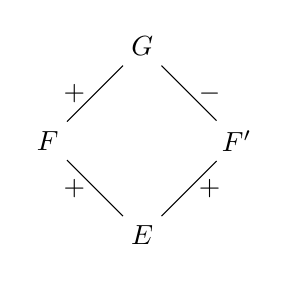
\begin{tikzpicture}[scale = .6]
	% Nodes
	\node (A) at (0,2) {$F$};
	\node (B) at (2,4) {$G$};
	\node (C) at (4,2) {$F'$};
	\node (D) at (2,0) {$E$};

	% Arrows
	\draw[-] (A) -- (B) node[midway, left] {$+$};
	\draw[-] (A) -- (D) node[midway, left] {$+$};
	\draw[-] (B) -- (C) node[midway, right] {$-$};
	\draw[-] (D) -- (C) node[midway, right] {$+$};
\end{tikzpicture}
\qquad
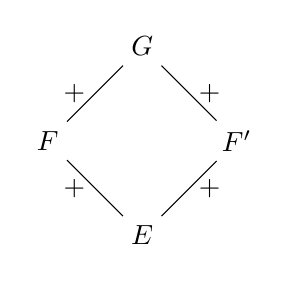
\begin{tikzpicture}[scale = .6]
	% Nodes
	\node (A) at (0,2) {$F$};
	\node (B) at (2,4) {$G$};
	\node (C) at (4,2) {$F'$};
	\node (D) at (2,0) {$E$};

	% Arrows
	\draw[-] (A) -- (B) node[midway, left] {$+$};
	\draw[-] (A) -- (D) node[midway, left] {$+$};
	\draw[-] (B) -- (C) node[midway, right] {$+$};
	\draw[-] (D) -- (C) node[midway, right] {$+$};
\end{tikzpicture}